% -------------------------------------------------------
% Results
% -------------------------------------------------------

\section{Results}

Our initial literature search retrieved 1981 articles, of which 454 remained after screening of the title and abstract. Following a more detailed evaluation of whether studies were on decision making and used eye-tracking, we identified 291 articles as potentially eligible studies. Based on detailed inspection of their full texts, 58 articles satisfied all inclusion criteria and were included in the meta-analysis. Figure~\ref{fig:flow_diagram} illustrates the PRISMA flow diagram \citep{moher2009preferred}. Many of the articles consisted of multiple experiments and some experiments operationalized more than one factor. This resulted in 106 independent effect size estimates, out of which 39 were effects of visual factors and 67 were effects of cognitive factors.

\begin{figure}[H]
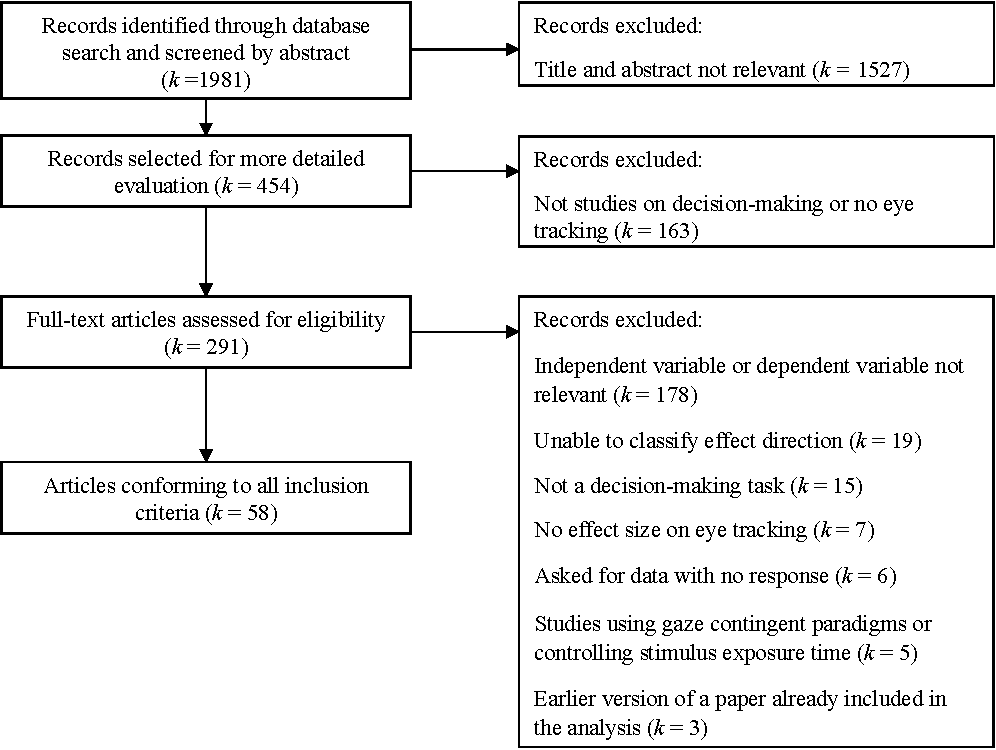
\includegraphics[width=0.8\textwidth]{prisma}
\centering
\caption{The PRISMA flow diagram showing the results of the literature search.}
\label{fig:flow_diagram}
\end{figure}


Meta-analyses of eye movements are relatively rare and it could be due to some methodological challenges in combining effect sizes from different eye-tracking studies. Two main challenges are how to handle measurement validity across eye-tracker types and how to compare different eye movement dependent variables. To handle these issues, we developed correction procedures to be integrated in a psychometric meta-analysis \citep{hunter2004a}, which allows us to quantify the interference of measurement validity or multiple metrics. The measurement validity issue stems from differences in the accuracy and precision of eye-tracking equipment \citep{holmqvist2015a}, which can affect the data quality and bias effect sizes \citep{orquin2016a}. We developed a correction method that relies on an empirical estimate of the relationship between eye-tracker characteristics and observed effect sizes (see \textit{Methods}; Figure~\ref{fig:ET_accuracy_effectsize}; Table~\ref{tab:eyetracker_specifications}) since there are multiple eye movement dependent variables commonly used. Most metrics are based on fixations -- defined as maintaining the gaze on a single location or area of interest (AOI), such as fixation count, fixation likelihood, total fixation duration and so on. This leads to a potential issue with comparing effect sizes reported with different dependent variables. We developed a correction method that makes the dependent variables comparable, where we empirically estimate correction factors based on a subset of studies in our sample that report multiple dependent variables (see \textit{Methods}; Figure~\ref{fig:metric_correction}; Table~\ref{tab:metric_correction}). This method allowed us to transform all effect sizes to a single metric; we decided for fixation count which was used in all meta-analyses. 

In what follows, we first analyse the group of visual factors and then the group of cognitive factors. We perform meta-analysis on each individual factor  separately. We next perform a small moderator analysis and finish with an analysis of publication bias in all the meta-analyses.  


\subsection{Visual factors}

We focused on four major groups of visual factors -- salience, position, surface size and set size (see \textit{Methods} for coding procedure). The summary effects of the visual factors on attention during decision making show that, except for salience and left vs right position, all factors have medium effect sizes ranging from $\rho=0.11$ to $\rho=0.695$, with moderate amounts of heterogeneity ranging from $I^2=0$ to $I^2=80.619$ (Table~\ref{tab:main_results} and Figure~\ref{fig:forest_plots_visual}). 
Salience, which so far has been taking the central stage in vision science, surprisingly has the smallest summary effect ($\rho=0.11$; 95\% confidence interval (CI) = $[-0.02,0.24]$; $p=0.098$), practically indistinguishable from a null effect. When we adjust the summary effect using the trim and fill method (see \textit{Publication bias} section), one imputed study decreases the effect size to ($\rho=0.18$; 95\% CI = $[0.12,0.25];$ Table~\ref{tab:main_results}). 
The position factor was decomposed into a left-vs-right (reading direction) and a center factor (tendency to attend to the center of the visual field). The center factor has the largest summary effect among visual factors ($\rho=0.43$; 95\% CI = $[0.26,0.59]$; $p< 0.001$), which decreases somewhat after the trim and fill adjustment ($\rho=0.39$; 95\% CI = $[0.22,0.56]$; $p< 0.001$; Table~\ref{tab:main_results}). 

Overall, three factors show reliable effect sizes: center position, surface size and set size. Considering that there is no (natural) environment free of visual factors, it is reasonable to expect that multiple visual factors influence eye movements at the same time. Hence, even though individual effect sizes are not large, jointly they can be a major driver of attention during decision making.


% \caption{Main results of the meta-analysis divided into independent variable subgroups }
% \label{tab:main_results}
% latex table generated in R 3.6.3 by xtable 1.8-4 package
% Sat Jun 20 12:32:29 2020
\begin{table}[ht]
\centering
\caption{Main results of the meta-analysis, divided into visual and cognitive factor groups, and individual factors within them. The most important values are the corrected effect size estimate, $\rho$, and the associated heterogeneity, $I^2$. Results of trim and fill analysis are in the parentesis.} 
\label{tab:main_results}
\begingroup\small
\begin{tabular}{lp{0.03\linewidth}p{0.05\linewidth}p{0.07\linewidth}p{0.07\linewidth}p{0.07\linewidth}p{0.07\linewidth}p{0.07\linewidth}p{0.07\linewidth}p{0.07\linewidth}}
  \hline
Group & $k$ & $N$ & $\rho$ & SE & $Z$ & $p$ & $\textrm{CI}_{95}$ LL & $\textrm{CI}_{95}$ UL & $I^2$ \\ 
  \hline
\textbf{Visual factors} &  &  &  &  &  &  &  &  &  \\ 
  Salience & 9 (1) & 530 & 0.11 (0.11) & 0.066 (0.121) & 1.659 (0.911) & 0.097 (0.362) & -0.02 (-0.127) & 0.24 (0.335) & 0 \\ 
  Surface size & 6 (0) & 740 & 0.396 (0.508) & 0.108 (0.188) & 3.682 (2.986) & 0 (0.003) & 0.185 (0.19) & 0.607 (0.73) & 55.31 \\ 
  Left vs right position & 3 (0) & 415 & 0.316 (0.485) & 0.213 (0.32) & 1.484 (1.652) & 0.138 (0.099) & -0.101 (-0.098) & 0.733 (0.82) & 46.04 \\ 
  Center position & 11 (0) & 912 & 0.434 (0.622) & 0.086 (0.209) & 5.065 (3.48) & 0 (0.001) & 0.266 (0.308) & 0.602 (0.814) & 49.92 \\ 
  Set size & 10 (0) & 610 & 0.29 (0.348) & 0.094 (0.126) & 3.095 (2.891) & 0.002 (0.004) & 0.106 (0.116) & 0.473 (0.544) & 55.06 \\ 
  \textbf{Cognitive factors} &  &  &  &  &  &  &  &  &  \\ 
  Task instructions & 26 (0) & 1990 & 0.419 (0.516) & 0.059 (0.084) & 7.146 (6.789) & 0 (0) & 0.304 (0.385) & 0.534 (0.626) & 43.75 \\ 
  Preferential viewing & 21 (0) & 2014 & 0.476 (0.75) & 0.086 (0.171) & 5.544 (5.677) & 0 (0) & 0.308 (0.563) & 0.645 (0.864) & 79.87 \\ 
  Choice bias & 18 (6) & 625 & 0.695 (0.949) & 0.086 (0.263) & 8.088 (6.929) & 0 (0) & 0.527 (0.863) & 0.864 (0.981) & 67.51 \\ 
   \hline 
 \multicolumn{10}{p{0.9\textwidth}}{\scriptsize{\textit{Note.} $k$ = number of studies (for trim and fill analysis number of imputed studies); $N$ = number of participants; $\rho$ = unattenuated effect size estimate, SE = standard error of estimate; $Z$ = Z statistic; $p$ = significance level; $\textrm{CI}_{95}$ LL = lower limit of the 95\% confidence interval; $\textrm{CI}_{95}$ UL = upper limit of the 95\% confidence interval, $I^2$ = within-group heterogeneity.}} 
\end{tabular}
\endgroup
\end{table}


\begin{figure}[!h]
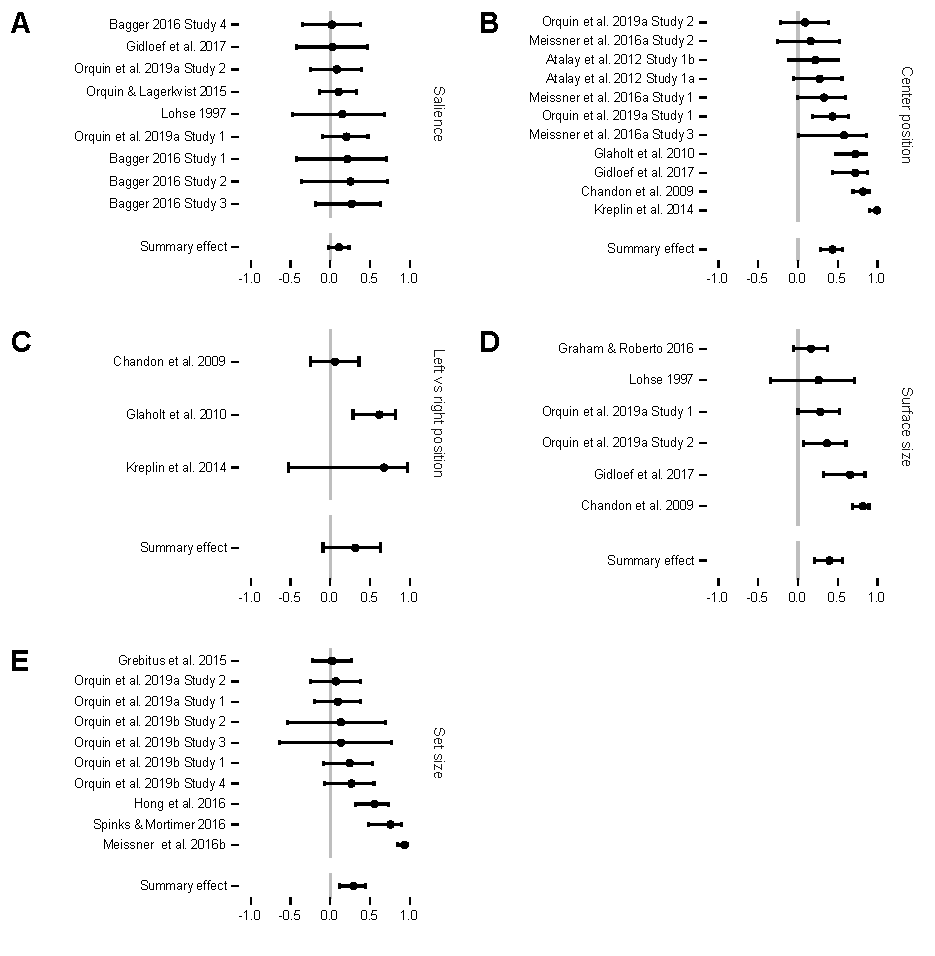
\includegraphics{forest_plots_visual}
\centering
\caption{Effect sizes of the visual factors are moderate, except for salience and left-vs-right position, which have small effect sizes, if any. Forest plots show the unattenuated effect size correlations for each study in a group, as well as average effect across the group. Forest plot in (A) shows the effect sizes for salience factor, in (B) for center position, in (C) for left vs right position, in  (D) for surface size, and in (E) for set size factor. Error bars represent the 95\% confidence interval around the mean.}
\label{fig:forest_plots_visual}
\end{figure}

\subsection{Cognitive factors}

Previous research has identified a wide range of cognitive factors that influence attention, such as goals, task instructions, and preferences \citep[for a review see][]{orquin2013a}. Here, we divided cognitive control factors into three groups: task instruction, preferential viewing and choice bias. 

In studies on task instructions, participants receive instructions concerning a specific decision goal, and with that, what is relevant to gaze at. For instance, the participants may be instructed on the validity of stimulus attributes \citep{krefeld-schwalb2019a}, or infer the level of validity themselves \citep{bialkova2014a}. In preferential viewing studies, the relevance should be equal to the subjective preferences. For example, some alternatives have higher subjective values than others \citep{kim2012a}. Because of this qualitative difference between the two domains, we treated studies on task instructions and preferential viewing separately. 
The inspection of the effect sizes reveals that the summary effects in the two types of studies are moderate and similar in magnitude -- in task instructions ($\rho=0.35$; 95\% CI = $[0.25,0.46]$; $p< 0.001$) 
and in preferential viewing ($\rho=0.46$; 95\% CI = $[0.29,0.63]$; $p< 0.001$; Table~\ref{tab:main_results} and Figure~\ref{fig:forest_plots_cognitive}). Using a Wald test, we find that effect sizes of task instructions and preferential viewing are unlikely to differ, $z=-0.033$, $p=0.399$. 
When we adjust the effects for publication bias using the trim and fill method, the effect size for task instructions decreases to ($\rho=0.32$; 95\% CI = $[0.21,0.44]$; $p< 0.001$; Table~\ref{tab:main_results}) and for preferential viewing to ($\rho=0.26$; 95\% CI = $[0.1,0.43]$; $pp=0.002$; Table~\ref{tab:main_results}). This result suggests that it makes no difference to eye movements whether the relevance of information is defined according to an externally specified goal or according to preferences. 

Choice bias refers to an effect in attention whereby decision makers spend more time gazing at the eventually chosen alternative. This effect, originally introduced by Shimojo and colleagues \citep{shimojo2003a} as a ``gaze-cascade'' effect, is well-established in the literature, prompting us to study it as a separate factor. This factor consists of studies reporting the difference in eye movements between the chosen alternative and all other (not chosen) alternatives. We find that choice bias has a large effect on eye movements, ($\rho=0.7$; 95\% CI = $[0.53,0.86]$; $p< 0.001$; Table~\ref{tab:main_results} and Figure~\ref{fig:forest_plots_cognitive}). The effect decreases to moderate size after publication bias adjustment ($\rho=0.41$; 95\% CI = $[0.22,0.59]$; $p< 0.001$; Table~\ref{tab:main_results})


\begin{figure}[!h]
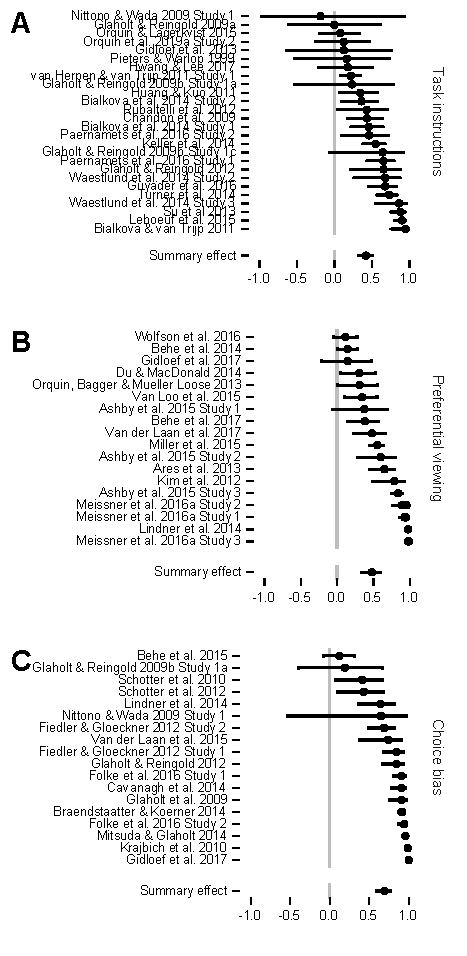
\includegraphics{forest_plots_cognitive}
\centering
\caption{Effect sizes of the three cognitive factors are moderate to large. Forest plots show the unattenuated effect size correlations for each study in a group, as well as average effect across the group. Forest plot in (A) shows the effect sizes for task instructions factor, in (B) for preferential viewing, and in (C) for the choice bias factor. Error bars represent the 95\% confidence interval around the mean.}
\label{fig:forest_plots_cognitive}
\end{figure}


\subsection{Moderator analyses}

Alternatives that participants in judgment and decision making studies choose between can often be decomposed into constituent elements, commonly called attributes, cues or features \citep{payne1988,tversky1972elimination,stojic2020s,gigerenzer1996reasoning,schulz2018putting,hogarth2007heuristic}. For example, in classical lottery tasks \citep{tversky1979}, the probabilities and values of an alternative can be viewed as attributes. Or, in multi-cue judgment tasks, alternatives are more explicitly composed of cues -- university, major football team or main city in the German city size task \citep{gigerenzer1996reasoning}. This has consequences for both modelling of decision processes and units of analysis. Consequently, some studies in our sample focused on attention effects at either alternative or attribute level, or both. This was in particular the case for studies involving set size, task instructions, and preferential viewing factors. Since the alternative vs attribute dimension might be an important moderator in these groups, we decomposed them further with regards to the effect of alternatives vs attributes (Table~\ref{tab:mod_results} and Figure~\ref{fig:forest_plots_altatt}). Moderator analyses shows a support for the alternative vs attribute moderator across set size, $Q_M(1)=4.765$, $p=0.029$, weak support for preferential viewing, $Q_M(1)=4.312$, $p=0.038$, and no support for task instructions, $t=-0.213$, $p=0.835$. It is noteworthy that effect sizes are consistently larger when operationalized at the level of alternatives compared to attributes (Table~\ref{tab:mod_results} and Figure~\ref{fig:forest_plots_altatt}). 

We also performed a moderator analysis for the choice bias factor, to assess whether the effect is driven by preferential viewing as proposed by \cite{shimojo2003a}. We compare studies with preferential vs inferential choice tasks and find no support for moderation by decision type, $Q_M(1)=0.057$, $p=0.811$, and only report results for the main group. 

\subsection{Publication bias}

We assessed potential publication bias using trim and fill analysis of each factor \citep{duval2000trim}. In addition, we plotted the  Fisher transformed correlation coefficients of each study by its respective standard error (so-called funnel plots; Figure~\ref{fig:funnel_plots} for main results, and Figure~\ref{fig:funnel_plots_altatt} for moderator analyses). The symmetry of the funnel plots provides a qualitative picture of whether there is a file drawer problem. We expect that studies with smaller sample sizes and hence higher standard errors yield more variable effect sizes, the smallest of which are less likely to be published, leading to an asymmetric funnel plot. Judging from the funnel plots, it is not obvious whether there is a problem with publication bias. However, the trim and fill analysis resulted in a downward adjustment of the average effect size for most of the factors. The corrected effect sizes in Table~\ref{tab:main_results} (in parentheses) provide a more conservative estimate of the true population effects, but are also subject to some uncertainty. Specifically, the interpretation of the corrected results may be biased due to heterogeneity in many of the factors as well as a relatively small number of studies in the group of visual factors. 


\begin{figure}[!h]
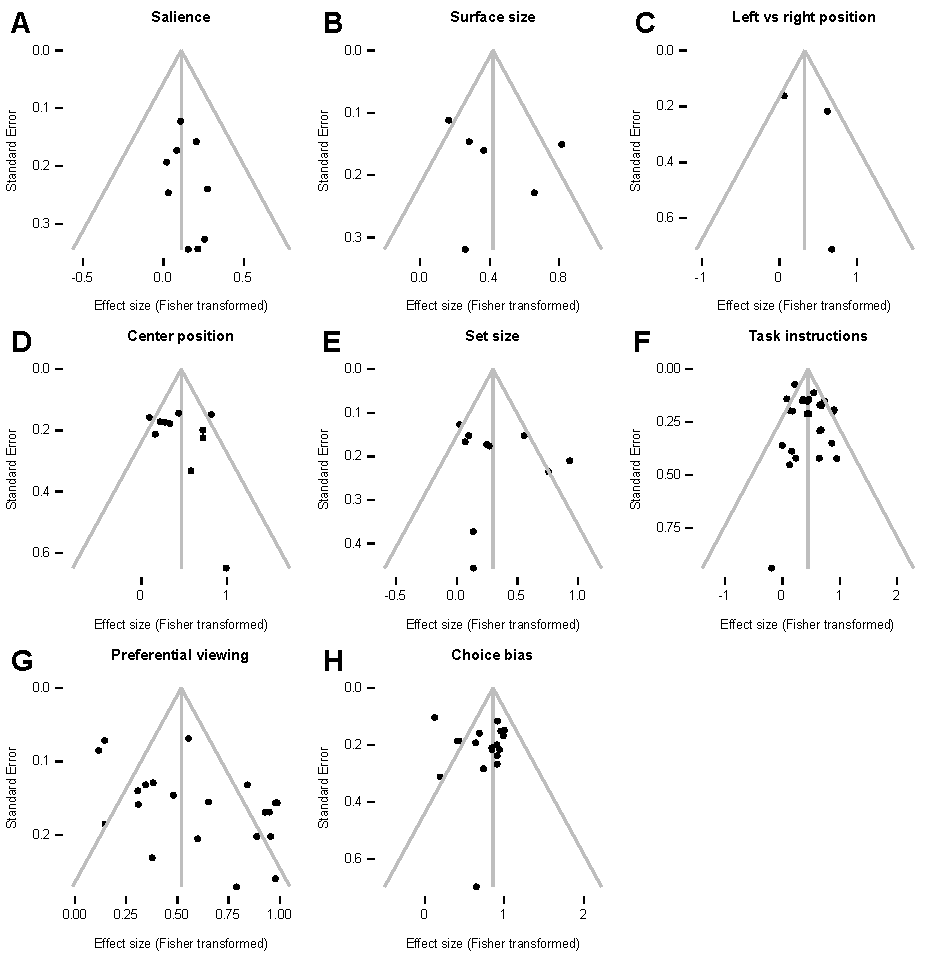
\includegraphics{funnel_plots}
\centering
\caption{Funnel plots for each factor that can be used as a qualitative check of a publication bias. Points are Fisher transformed correlation coefficients against their standard error. Asymmetric distributions of points can indicate the presence of publication bias since smaller studies (those with higher standard errors) have more variable effect sizes and are less likely to be published unless the effect is large. Funnel plot for (A) salience, (B) surface size, (C) left vs right position, (D) central position, (E) set size, (F) task instructions, (G) preferential viewing, and (H) choice bias.}
\label{fig:funnel_plots}
\end{figure}

\chg{EM section}{
\subsection{Descriptive eye movement data}
To better understand the results of the meta-analysis we extract for each effect size the corresponding descriptive eye movement data whenever the included article reports this information.} 

\begin{figure}[!h]
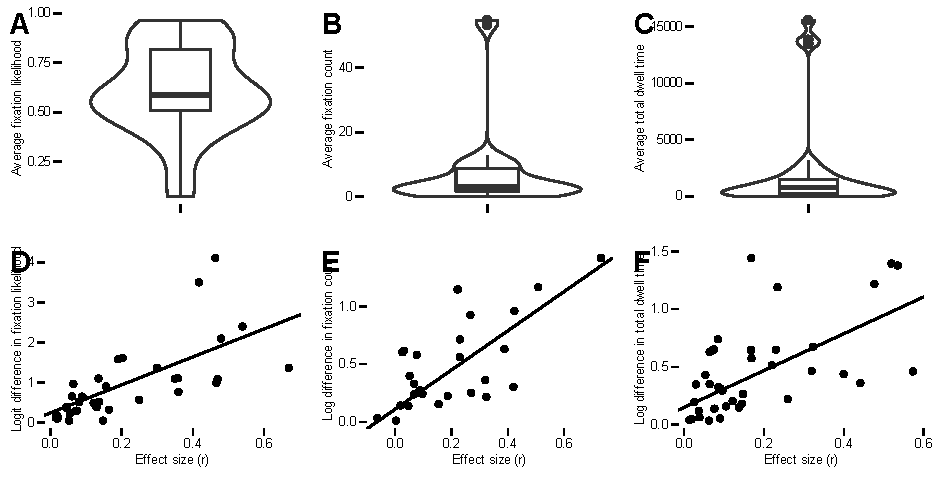
\includegraphics{figs/EMtoES.pdf}
\centering
\caption{}
\label{fig:em_figure}
\end{figure}